%\chapter{Ergebnisse}
\section{Ergebnisse der Actionserkennung}
\label{sec:ergebnisse}
Es wurde ein Datenset erstellt welches aus 80\% selbst aufgenommen Videos und 20\% Videos aus der Uni Clinc Heidelberg.


Es wurde ein Neuronales Netz zur Action Erkennung gefunden. Für dieses Netz wurden Python Skripte erstellt, welche die Trainingsdaten so vor verarbeiten, dass damit ein Netz trainiert werden konnte. Anschließend wurde das 3D-ConvNet mit 6 Klassen: Gloves on, cleaning, unpacking, Gloves off, disinfekt, others mit jeweils 40 Videos trainiert. Die Evaluation gab gute Ergebnisse aus, das Netz hat eine Pression von 90\% erreichen. Mit diesen Ergebnissen konnte man zeigen, dass es möglich ist diese Netzstruktur für Ego-Action-Recognition zu verwenden.


\section{Verbesserungsvorschläge und Zukunftsaussicht}
\label{sec:Verbesserungen}

\subsubsection{Erweiterung der Trainingsdaten}
Die Trainerdaten können noch erweitert werden, einmal mit Realen Daten und weitern Klassen.
Oder mit Data-Argumentation, in welcher man durch Drehen oder einbringen von Farben künstlich mehr Daten erstellt und somit eine bessere Erkennung zubekommen.

\subsubsection{Realtime-Anwendung}
Die Schnelligkeit muss verbessert werden und die API muss angepasst werden, um es als Realtimeanwendung umsetzen zukönnen.
Dies übersteigt aber die Zeit in meinem Praktikum und ist deswegen noch zu entwickeln.

\subsubsection{Optical Flow}
Der Optical Flow wurde umgesetzt, dennoch ist es möglich, diesen zu Verbessern, durch verschiedene Vorverarbeitungen z.b. Bildstabilisierungen. Dies ist nicht getestet worden, könnte aber zu Verbesserungen führen, um Hintergrundstörungen aus den einzelnen Images zu filtern.

\subsubsection{Dritter Steam mit Händen}
Des Weiteren könnte man das Netz mit einem dritten Steam erweitern, um so den Focus auf spezielle Details zu legen.

\begin{itemize}

\item \textbf{Segmentation der Hände:}
Mit der Segmentation der Hände wäre es möglich speziellen Focus auf die Hände zulegen oder auf Video abschnitte mit Händen.

\begin{figure}[!htb]
  \centering
  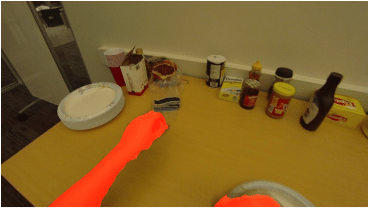
\includegraphics[scale=0.5]{img/hands.png}
  \caption{Segmentation Hands  \cite{Bambach_2015_ICCV}}
  \label{fig:Optical FLow}
\end{figure}

\item \textbf{Hand-Pose:}
Mit der Pose Estimation der Hände wäre eine Weiterentwicklung der Segmentation. Mit der Pose Estimation der Hände wäre eine Weiterentwicklung der Segmentation. Dennoch wurde dies meist mit RGB-D Images umgesetzt. RGB-D Images enthalten noch weiter Tiefeninformation welche die GoPro nicht mit liefert.

\begin{figure}[!htb]
  \centering
  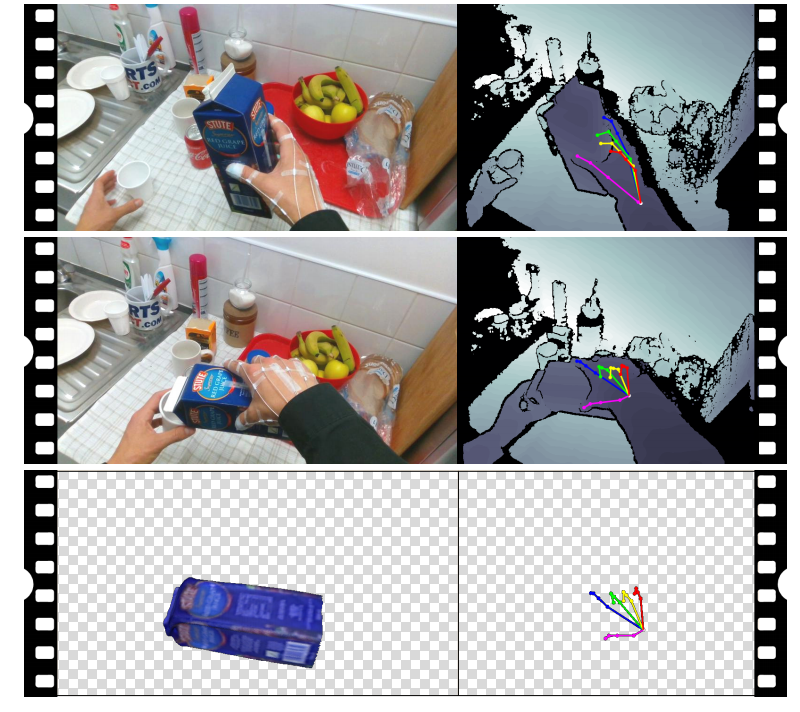
\includegraphics[scale=0.25]{img/Hand-Pose.png}
  \caption{Hand-Pose with RGB-D-Images   \cite{Hand-Pose-paper}}
  \label{fig:Optical Flow}
\end{figure}

\end{itemize}
